%%%%%%%% ICML 2021 EXAMPLE LATEX SUBMISSION FILE %%%%%%%%%%%%%%%%%

\documentclass{article}

% Recommended, but optional, packages for figures and better typesetting:
\usepackage{microtype}
\usepackage{graphicx}
\usepackage{subfigure}
\usepackage{booktabs} % for professional tables

% hyperref makes hyperlinks in the resulting PDF.
% If your build breaks (sometimes temporarily if a hyperlink spans a page)
% please comment out the following usepackage line and replace
% \usepackage{icml2021} with \usepackage[nohyperref]{icml2021} above.
\usepackage{hyperref}

% Attempt to make hyperref and algorithmic work together better:
\newcommand{\theHalgorithm}{\arabic{algorithm}}

% Use the following line for the initial blind version submitted for review:
\usepackage{icml2021}

% If accepted, instead use the following line for the camera-ready submission:
%\usepackage[accepted]{icml2021}

% The \icmltitle you define below is probably too long as a header.
% Therefore, a short form for the running title is supplied here:
\icmltitlerunning{Nonparametric tensor completion}
\usepackage{mathrsfs}
\usepackage{wrapfig}
\usepackage{multirow}
\usepackage{graphicx}
%\usepackage[utf8]{inputenc} % allow utf-8 input
%\usepackage[T1]{fontenc}    % use 8-bit T1 fonts
\usepackage{hyperref}       % hyperlinks
\usepackage{url}            % simple URL typesetting
%\usepackage{booktabs}       % professional-quality tables
\usepackage{amsmath,amssymb}
\usepackage{amsthm}    % blackboard math symbols
%\usepackage{nicefrac}       % compact symbols for 1/2, etc.
%\usepackage{microtype}      % microtypography
\usepackage{bm}
%\usepackage{subfig}
%\usepackage[english]{babel}
%\usepackage{algorithm}
%\usepackage{appendix}
\usepackage{mathtools}
\mathtoolsset{showonlyrefs}
\usepackage{enumitem}
\theoremstyle{plain}
\newtheorem{thm}{Theorem}
\newtheorem{lem}{Lemma}
\newtheorem{prop}{Proposition}
\newtheorem{pro}{Property}
\newtheorem{cor}{Corollary}

\theoremstyle{definition}
\newtheorem{defn}{Definition}
\newtheorem{assumption}{Assumption}
\newtheorem{example}{Example}
\newtheorem{rmk}{Remark}


\newtheorem{innercustomgeneric}{\customgenericname}
\providecommand{\customgenericname}{}
\newcommand{\newcustomtheorem}[2]{%
  \newenvironment{#1}[1]
  {%
   \renewcommand\customgenericname{#2}%
   \renewcommand\theinnercustomgeneric{##1}%
   \innercustomgeneric
  }
  {\endinnercustomgeneric}
}

\newcustomtheorem{customexample}{Example}




\usepackage{dsfont}
%\usepackage{algpseudocode,algorithm}
%\algnewcommand\algorithmicinput{\textbf{Input:}}
%\algnewcommand\algorithmicoutput{\textbf{Output:}}
%\algnewcommand\INPUT{\item[\algorithmicinput]}
%\algnewcommand\OUTPUT{\item[\algorithmicoutput]}
%\DeclareMathOperator*{\minimize}{minimize}

\usepackage{xr}



\newcommand*{\KeepStyleUnderBrace}[1]{%f
  \mathop{%
    \mathchoice
    {\underbrace{\displaystyle#1}}%
    {\underbrace{\textstyle#1}}%
    {\underbrace{\scriptstyle#1}}%
    {\underbrace{\scriptscriptstyle#1}}%
  }\limits
}
\usepackage{makecell}
\input macros.tex

\usepackage{amssymb}
\usepackage{pifont}
\def\sign{\textup{sgn}}
\def\srank{\textup{srank}}
\def\rank{\textup{rank}}
\def\caliP{\mathscr{P}_{\textup{sgn}}}
\def\risk{\textup{Risk}}

\usepackage{xr}
\externaldocument{signT_supp}

\begin{document}

\twocolumn[
\icmltitle{Beyond the Signs: Nonparametric Tensor Completion via Sign Series}

\icmlsetsymbol{equal}{*}

\begin{icmlauthorlist}
\icmlauthor{Chanwoo Lee}{wisc}
\icmlauthor{Miaoyan Wang}{wisc}
\end{icmlauthorlist}

\icmlaffiliation{wisc}{Department of Statistics, University of Wisconsin -- Madison}


\icmlcorrespondingauthor{Miaoyan Wang}{miaoyan.wang@wisc.edu}


% You may provide any keywords that you
% find helpful for describing your paper; these are used to populate
% the "keywords" metadata in the PDF but will not be shown in the document
\icmlkeywords{Higher-order tensors, completion, sliced inverse regression, probability estimation}

\vskip 0.3in
]

% this must go after the closing bracket ] following \twocolumn[ ...

% This command actually creates the footnote in the first column
% listing the affiliations and the copyright notice.
% The command takes one argument, which is text to display at the start of the footnote.
% The \icmlEqualContribution command is standard text for equal contribution.
% Remove it (just {}) if you do not need this facility.

\printAffiliationsAndNotice{}  % leave blank if no need to mention equal contribution


\begin{abstract}
We consider the problem of tensor estimation from noisy observations with possibly missing entries. A nonparametric approach to tensor completion is developed based on a new model which we coin as sign representable tensors. The model represents the signal tensor of interest using a series of structured sign tensors. Unlike earlier methods, the sign series representation effectively addresses both low- and high-rank signals, while encompassing many existing tensor models---including CP models, Tucker models, single index models, certain hypergraphon models---as special cases. We show that the sign tensor series are theoretically characterized, and computationally estimable, by classification tasks with carefully-specified weights. Excess risk bounds, estimation error rates, and sample complexities are established. We demonstrate the outperformance of our approach over previous methods on two datasets, one on human brain connectivity networks and the other on author-topic mining. 
\end{abstract}

\section{Introduction}\label{sec:intro}

Higher-order tensors have recently received much attention in enormous fields including social networks~\cite{anandkumar2014tensor}, neuroscience~\cite{wang2017bayesian}, and genomics~\cite{wang2019three}. Tensor methods provide effective representation of the hidden structure in multiway data. In this paper we consider the signal plus noise model,
\begin{equation}\label{eq:modelintro}
\tY=\Theta+\tE,
\end{equation}
where $\tY\in\mathbb{R}^{d_1\times \cdots \times d_K}$ is an order-$K$ data tensor, $\Theta$ is an unknown signal tensor of interest, and $\tE$ is the noise tensor. Our goal is to accurately estimate $\Theta$ from the incomplete, noisy observation of $\tY$. In particular, we focus on the following two problems:
\begin{itemize}[leftmargin=*,topsep=0pt,itemsep=-1ex,partopsep=1ex,parsep=1ex]
\item Q1 [Nonparametric tensor estimation]. How to flexibly estimate $\Theta$ under a wide range of structures, including both low-rankness and high-rankness?
\item Q2 [Tensor completion]. How many observed tensor entries do we need to consistently estimate the signal $\Theta$?
\end{itemize}

%\subsection{Inadequacies of common low-rank models}\label{sec:example}
{\bf Inadequacies of common low-rank models.} The signal plus noise model~\eqref{eq:model} is popular in tensor literature. Existing methods perform estimation based on low-rankness of $\Theta$~\cite{montanari2018spectral,cai2019nonconvex}. Common low-rank models include CP tensors~\cite{anandkumar2014tensor}, Tucker tensors~\cite{de2000multilinear}, and block tensors~\cite{wang2019multiway}. While these methods have shown great success in signal recovery, tensors sought in application often violate the low-rankness. Here we provide two examples to illustrate the limitation of classical models.

\begin{figure}[h]
\vspace{-.2cm}
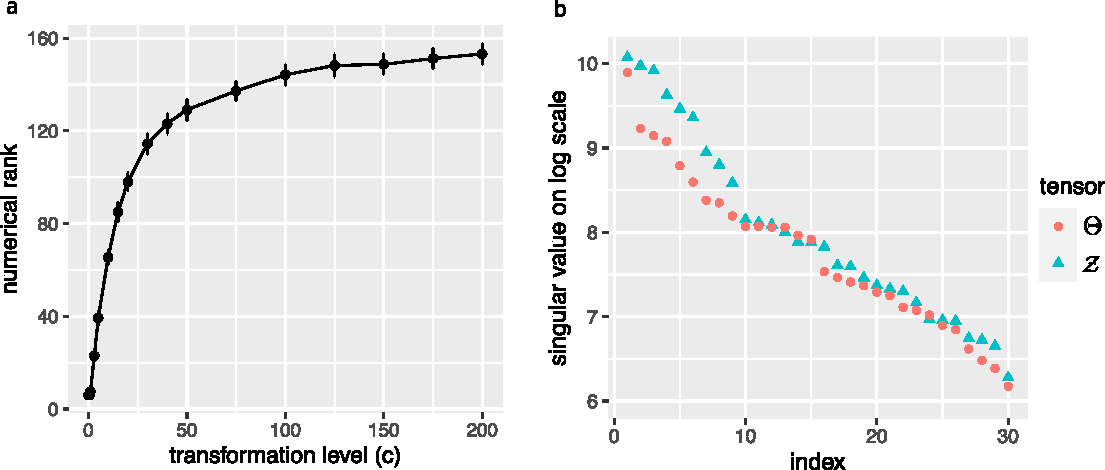
\includegraphics[width=.47\textwidth]{figure/example_comb.pdf}
\caption{(a) Numerical rank of $\Theta$ versus $c$ in the first example. (b) Top $d=30$ tensor singular values in the second example. }\label{fig:example}
\vspace{-.3cm}
\end{figure}

\begin{figure*}[h!]
\vspace{-.2cm}
\centerline{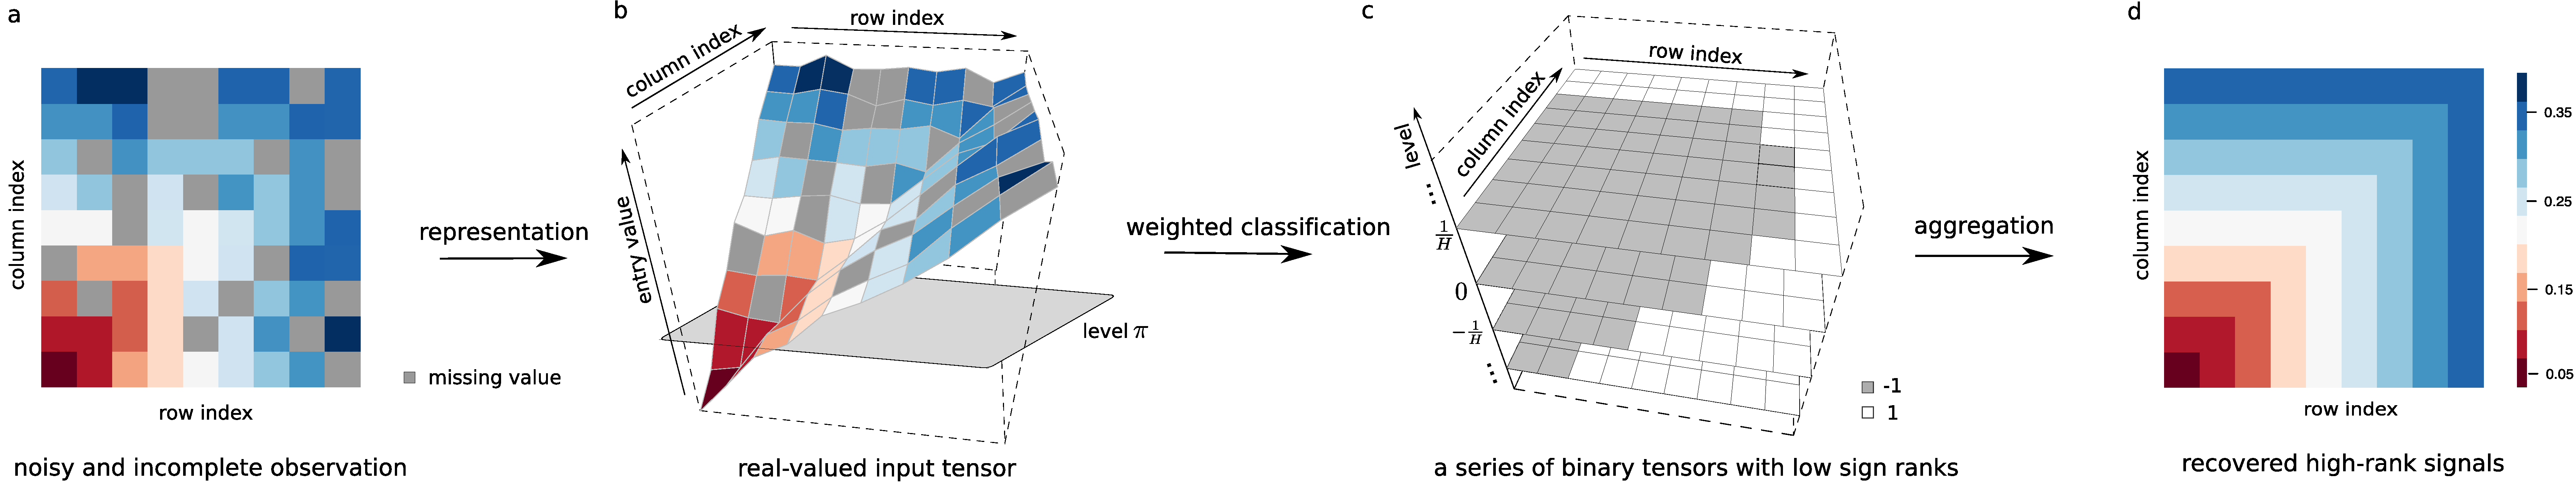
\includegraphics[width=1\textwidth]{figure/image_new2.pdf}}
\caption{Illustration of our method. For visualization purpose, we plot an order-2 tensor (a.k.a.\ matrix); similar procedure applies to higher-order tensors. (a): noisy and incomplete tensor input. (b) and (c): main steps of estimating sign tensor series $\sign(\Theta-\pi)$ for all $\pi\in {\scriptstyle  \{-1,\ldots,-{1\over H},0,{1\over H},\ldots,1\}}$. (d) estimated signal $\hat \Theta$. The depicted example is a full-rank signal matrix based on Example 5 in Section~\ref{sec:representation}.}\label{fig:demo}
\vspace{-.4cm}
\end{figure*}

The first example reveals the sensitivity of tensor rank to order-preserving transformations. Let $\tZ \in \mathbb{R}^{30\times 30\times 30}$ be an order-3 tensor with CP $\text{rank}(\tZ)=3$ (formal definition is deferred to end of this section). Suppose a monotonic transformation $f(z)=(1+\exp(-cz))^{-1}$ is applied to $\tZ$ entrywise, and we let the signal $\Theta$ in model~\eqref{eq:modelintro} be the tensor after transformation. Figure~\ref{fig:example}(a) plots the numerical rank of $\Theta$ versus $c$. As we see, the rank increases rapidly with $c$, rending traditional low-rank tensor methods ineffective even in the presence of mild order-preserving nonlinearities. In applications of digital processing~\cite{karbasi2012robust} and genomics analysis~\cite{wang2019three}, the tensor of interest often undergoes unknown transformation prior to measurements. The sensitivity to transformation makes the low-rank model less desirable in practice. 

The second example demonstrates the inadequacy of classical low-rankness in representing important special structures. Here we consider the signal tensor of the form $\Theta=\log(1+\tZ)$, where $\tZ\in\mathbb{R}^{d\times d\times d}$ is an order-3 tensor with entries $\tZ(i,j,k)={1\over d}\max(i,j,k)$ for $i,j,k\in\{1,\ldots,d\}$. The matrix analogy of $\Theta$ was studied in~\citet{chan2014consistent} as graph functions. In this case neither $\Theta$ nor $\tZ$ is low-rank; in fact, the rank is no smaller than the dimension $d$ as illustrated in Figure~\ref{fig:example}(b). Again, classical low-rank models fail to address this type of tensor structure. 

In the above and many other examples, the signal tensors $\Theta$ of interest have high rank. Classical low-rank models will miss these important structures. New methods that allow flexible tensor modeling have yet to be developed. 

{\bf Our contributions.}
We develop a new model called sign representable tensors to address the aforementioned challenges. 
Figure~\ref{fig:demo} illustrates our main idea. Our approach is built on the nonparametric sign representation of signal tensors, and we propose to estimate the sign tensors through a series of weighted classifications. In contrast to existing methods, our method is guaranteed to recover a wide range of low- and high-rank signals. We highlight two main contributions that set our work apart from earlier literature. 

Statistically, the problem of high-rank estimation is fundamentally challenging. Existing estimation theory~\cite{montanari2018spectral,cai2019nonconvex,ghadermarzy2019near} exclusively focuses on the regime of fixed $r$ growing $d$. However, such premise fails in high-rank tensors, where the rank may grow with, or even exceed, the dimension. A proper notion of nonparametric complexity is crucial. We show that, somewhat surprisingly, the sign tensor series not only preserves all information in the original signals, but also brings the benefits of flexibility and accuracy over classical low-rank models. The results fill the gap between parametric (low-rank) and nonparametric (high-rank) tensors, thereby greatly enriching the tensor literature. 

From computational perspective, optimizations regarding tensors are in general NP-hard. Fortunately, tensors sought in application are often specially-structured, for which a number of efficient algorithms are available~\cite{ghadermarzy2018learning,wang2018learning, han2020optimal}. Our high-rank tensor estimate is provably reductable to a series of classifications, and it enjoys the divide-and-conquer nature that facilitates computation. The ability to import and adapt existing tensor algorithms is one advantage of our method. 

We also highlight the challenges associated with tensors compared to matrices. High-rank matrix estimation is recently studied under nonlinear models~\cite{ganti2015matrix} and subspace clustering~\cite{pmlr-v70-ongie17a,fan2019online}. However, the problem for high-rank tensors is more prevalent, because the tensor rank often exceeds the dimension when order $K\geq 3$~\cite{anandkumar2017analyzing}. This is in sharp contrast to matrices. We show that, applying matrix methods to higher-order tensors results in suboptimal estimates. A full exploitation of the higher-order structure is needed; this is another challenge we address in this paper.


{\bf Notation.}
We use $\sign(\cdot)\colon \mathbb{R}\to\{-1,1\}$ to denote the sign function, where $\sign(y)=1$ if $y\geq 0$ and $-1$ otherwise. We allow univariate functions, such as $\sign(\cdot)$ or general $f\colon \mathbb{R}\to\mathbb{R}$, to be applied to tensors in an element-wise manner. 
We denote $a_n\lesssim b_n$ if $\lim_n b_n/a_n\rightarrow 0.$ We use the shorthand $[n]$ to denote the $n$-set $\{1,\ldots,n\}$ for $n\in\mathbb{N}_{+}$. Let $\tY\in\mathbb{R}^{d_1\times \cdots \times d_K}$ denote an order-$K$ $(d_1,\ldots,d_k)$-dimensional tensor, and $\tY(\omega)\in\mathbb{R}$ denote the tensor entry indexed by $\omega \in[d_1]\times \cdots \times [d_K]$. An event $E$ is said to occur ``with high probability'' if $\mathbb{P}(E)$ tends to 1 as the tensor dimension $d_{\min}=\min_k d_k \to\infty$. The Canonical Polyadic (CP) decomposition~\cite{hitchcock1927expression} for a tensor $\Theta\in\mathbb{R}^{d_1\times \cdots \times d_K}$ is defined as
\begin{equation}\label{eq:CP}
\Theta=\sum_{s=1}^r\lambda_s \ma^{(1)}_s\otimes\cdots\otimes \ma^{(K)}_s,
\end{equation}
where $\lambda_1\geq \cdots \geq \lambda_r>0$ are called tensor singular values, and $\ma^{(k)}_s$ are norm-1 tensor singular vectors, for all $s\in[r]$, $k\in[K]$, and $\otimes$ denote the outer product of vectors.
The minimal $r$ for which the decomposition~\eqref{eq:CP} holds is called the tensor rank, denoted as $\rank(\Theta)$. 


\section{Model and proposal overview}\label{sec:overview}

Let $\tY$ be an order-$K$ $(d_1,\ldots,d_K)$-dimensional data tensor generated from the following model,
\begin{equation}\label{eq:model}
\tY=\Theta+\tE,
\end{equation}
where $\Theta\in\mathbb{R}^{d_1\times \cdots \times d_K}$ is the unknown signal tensor of interest, and $\tE$ is a noise tensor consisting of mean-zero, independent but not necessarily identically distributed entries. We allow heterogenous noise such that the marginal distribution of noise entry $\tE(\omega)$ may depend on $\omega$. In general, assume that $\tY(\omega)$ take values in a bounded interval $[-A, A]$. We assume $A=1$ throughout the paper. 

Our observation is an incomplete data tensor from~\eqref{eq:model}, denoted $\tY_\Omega$, where $\Omega\subset[d_1]\times\cdots\times[d_K]$ is the index set of observed entries. We consider a general model on $\Omega$ that allows both uniform and non-uniform samplings. Specifically, let $\Pi=\{\pi_\omega\}$ be an arbitrarily predefined probability distribution over the full index set with $\sum_{\omega\in[d_1]\times \cdots \times [d_K]}\pi_\omega=1$. Assume that the entries $\omega$ in $\Omega$ are i.i.d.\ draws with replacement from the full index set using distribution $\Pi$. The sampling rule will be denoted as $\omega\sim \Pi$.


Before describing our main results, we provide the intuition behind our method. In the two examples in Section~\ref{sec:intro}, the high-rankness in the signal $\Theta$ makes the estimation challenging. However, if we examine the sign of the $\pi$-shifted signal $\sign(\Theta-\pi)$ for any given $\pi$, then, these sign tensors share the same sign patterns as low-rank tensors. Indeed, the signal tensor in example 1 has the same sign pattern as a rank-$4$ tensor, since $\sign(\Theta-\pi)=\sign(\tZ-f^{-1}(\pi))$. The signal tensor in example 2 has the same sign pattern as a rank-2 tensor, since $\sign(\Theta-\pi)=\sign(\max(i,j,k)-d(e^{\pi}-1))$.


The above observation suggests a general framework to estimate both low- and high-rank signal tensors. Figure~\ref{fig:demo} illustrates the main crux of our method. We dichotomize the data tensor into a series of sign tensors, $\sign (\tY_\Omega-\pi)$, for all $\pi\in \tH={\{\small-1,\ldots,  -{1\over H},0, {1\over H},\ldots,1\}}$, and then estimate the sign signals, $\sign(\Theta-\pi)$, by performing classification
\[
\hat \tZ_\pi=\argmin_{\text{low rank tensor $\tZ$}} L(\sign(\tZ),\ \sign (\tY_\Omega-\pi)).
\]
Here, $L(\cdot,\cdot)$ denotes a carefully-designed classification objective function which will be described in later sections. Our final proposed tensor estimate takes the form
\[
\hat \Theta = {1\over 2H+1}\sum_{\pi \in \tH} \sign(\hat \tZ_\pi).
\]
Our approach is built on the nonparametric sign representation of signal tensors, and the estimate $\hat \Theta$ is essentially learned from dichotomized tensor series $\{\sign(\tY_\Omega-\pi)\colon \pi \in \tH\}$ with certain weights. Interestingly, we show that a proper analysis of dichotomized data not only preserves all information in the original signals, but also brings benefits of accuracy and flexibility over classical low-rank models. 
%The method enjoys both statistical effectiveness and computational efficiency. 



\section{Sign representable tensors}\label{sec:representation}
This section develops sign representable tensor models for $\Theta$ in~\eqref{eq:model}. We characterize the algebraic and statistical properties of sign tensor series, which serves the theoretical foundation for our method. 

\subsection{Sign-rank and sign tensor series}\label{sec:sign-rank}
Let $\Theta$ be a tensor of interest and $\sign (\Theta)$ the corresponding sign patten. The sign pattern induces an equivalence relationship between tensors. Two tensors are called sign equivalent, denoted $\simeq$, if they share the same sign patterns. 

\begin{defn}[Sign-rank]
The sign-rank of a tensor $\Theta\in\mathbb{R}^{d_1\times \cdots \times d_L}$ is the minimal rank among all tensors that share the same sign patterns as $\Theta$; i.e.,
\[
\srank(\Theta) = \min \{\rank(\Theta')\colon  \Theta'\simeq \Theta,\ \Theta'\in\mathbb{R}^{d_1\times \cdots \times d_K}\}.
\]
\end{defn}
The sign-rank is also called \emph{support rank}~\cite{cohn2013fast}, \emph{minimal rank}~\cite{alon2016sign}, and \emph{nondeterministic rank}~\cite{de2003nondeterministic}. Earlier work defines sign-rank for binary tensors/matrices only; we extend the notion to continuous-valued tensors. Note that the sign-rank concerns only the sign pattern but discards the magnitudes information of $\Theta$. In particular, $\srank(\Theta)=\srank(\sign \Theta)$. 

Like most tensor problems~\cite{hillar2013most}, determining the sign-rank for a general tensor is NP hard~\cite{alon2016sign}. Fortunately, tensors arisen in application often possess special structures that facilitate analysis. We show that the low sign-rank family is strictly broader than usual low-rank family. By definition, the sign-rank is upper bounded by the usual rank. More generally, 
\begin{prop}[Upper bounds of sign-rank]~\label{cor:monotonic} For any strictly monotonic function $g\colon \mathbb{R}\to \mathbb{R}$ with $g(0)=0$, 
\[
\textup{srank}(\Theta)\leq\rank(g(\Theta)).
\]
\end{prop}
Conversely, the sign-rank is often dramatically smaller than the usual rank, as we have shown in Section~\ref{sec:intro}.
\begin{prop}[Broadness]\label{prop:extention}For every order $K\geq 2$ and dimension $d$, there exist order-$K$ $(d,\ldots,d)$-dimensional tensors $\Theta$ such that $\rank(\Theta)=d$ and $\srank(\Theta)=2$.
\end{prop}
We provide several examples in Appendix, in which the tensor rank grows with dimension $d$ but the sign-rank remains a constant. The results highlight the advantages of using sign-rank in the high-dimensional tensor analysis. Corollary~\ref{cor:monotonic} and Proposition~\ref{prop:extention} together demonstrate the strict broadness of low sign-rank family over the usual low-rank family. 

We now introduce a tensor family, which we coin as ``sign representable tensors'', for the signal tensors in model~\eqref{eq:model}. 
\begin{defn}[Sign representable tensors] 
Fix a level $\pi\in[-1,1]$. A tensor $\Theta$ is called $(r,\pi)$-sign representable, if the tensor $(\Theta-\pi)$ has sign-rank bounded by $r$. A tensor $\Theta$ is called $r$-sign (globally) representable, if $\Theta$ is $(r,\pi)$-sign representable for all $\pi\in[-1,1]$. The collection $\{\sign(\Theta-\pi)\colon \pi \in[-1,1]\}$ is called the sign tensor series. 
We use $\caliP(r)=\{\Theta\colon \srank(\Theta-\pi)\leq r \text{ for all }\pi\in[-1,1]\}$ to denote the $r$-sign representable tensor family.
\end{defn}

We show that the $r$-sign representable tensor family is a general model that incorporates most existing tensor models, including low-rank tensors, single index models, GLM models, and certain hypergraphon models. 

\begin{example}[CP/Tucker low-rank models] The CP and Tucker low-rank tensors are the two most popular tensor models~\cite{kolda2009tensor}. Let $\Theta$ be a low-rank tensor with CP rank $r$. We see that $\Theta$ belongs to the sign representable family; i.e., $\Theta\in\caliP(r+1)$ (the constant $1$ is due to $\rank(\Theta-\pi)\leq r+1$). Similar results hold for Tucker low-rank tensors $\Theta\in\caliP(r+1)$, where $r=\prod_kr_k$ with $r_k$ being the $k$-th mode Tucker rank of $\Theta$.  
\end{example} 

\begin{example}[Tensor block models (TBMs)] Tensor block model~\cite{wang2019multiway,chi2020provable} assumes a checkerbord structure among tensor entries under marginal index permutation. The signal tensor $\Theta$ takes at most $r$ distinct values, where $r$ is the total number of multiway blocks. Our model incorporates TBM because $\Theta \in \caliP(r)$. 
\end{example}


\begin{example}[Generalized linear models (GLMs)] Let $\tY$ be a binary tensor from a logistic model~\cite{wang2018learning} with mean $\Theta=\text{logit}(\tZ)$, where $\tZ$ is a latent low-rank tensor. By definition, $\Theta$ is a low-rank sign representable tensor; note that $\Theta$ itself is a high-rank tensor (see Section~\ref{sec:intro}). Same conclusion holds for general exponential-family tensor mean with a (known) link function~\cite{hong2020generalized}. 
\end{example}

\begin{example}[Single index models (SIMs)] Single index model is a flexible semiparametric model proposed in economics~\cite{robinson1988root} and high-dimensional statistics~\cite{balabdaoui2019least,ganti2017learning}. We here extend the model to higher-order tensors $\Theta$. The SIM assumes the existence of a (unknown) monotonic function $g\colon \mathbb{R}\to \mathbb{R}$ such that $g(\Theta)$ has rank $r$. We see that $\Theta$ belongs to the sign representable family; i.e., $\Theta\in \caliP(r+1)$. 
\end{example}

\begin{example}[Min/Max hypergraphon] Graphon is a popular nonparametric model for networks~\cite{chan2014consistent,xu2018rates}. Here we revisit the model introduced in Section~\ref{sec:intro} for generality. Let $\Theta$ be an order-$K$ tensor generated from the hypergraphon $\Theta(i_1,\ldots,i_K)=\log(1+\max_kx^{(k)}_{i_k})$, where $x^{(k)}_{i_k}\sim \text{Unif}[0,1]$ i.i.d.\ for all $i_k\in[d_k]$ and $k\in[K]$. We conclude that $\Theta \in \caliP(2)$, because every sign tensor $\sign(\Theta-\pi)$ in the series of $\pi\in[0,\ \log 2]$ is a block tensor with at most two blocks.

The results extend to general min/max hypergraphons. Let $g(\cdot)$ be a continuous univariate function with at most $r\geq 1$ real-valued roots in the equation $g(z)=\pi$; this property holds, e.g., when $g(z)$ is a polynomial of degree $r$. Then, the tensor $\Theta$ generated from $\Theta(i_1,\ldots,i_K)=g(\max_kx^{(k)}_{i_k})$ belongs to $\caliP(r+1)$. Same conclusion applies if the maximum is replaced by minimum.
\end{example}

\subsection{Statistical characterization of sign tensors via weighted classification}\label{sec:identifiability}

Accurate estimation of a sign representable tensor depends on the behavior of sign tensor series, $\sign(\Theta-\pi)$. In this section, we show that sign tensors are completely characterizes by weighted classification. The results bridge the algebraic and statistical properties of sign representable tensors.
 
For a given $\pi \in [-1,1]$, define a $\pi$-shifted data tensor $\bar \tY_\Omega$ with entries $\bar \tY(\omega) = (\tY(\omega)-\pi)$ for $\omega\in \Omega$. We propose a weighted classification objective
\begin{equation}\label{eq:sample}
L(\tZ, \bar \tY_\Omega)= {1\over |\Omega|}\sum_{\omega \in \Omega}\KeepStyleUnderBrace{|\bar \tY(\omega)|}_{\text{entry-specific weight}} \times \KeepStyleUnderBrace{| \sign \tZ(\omega)-\sign \bar \tY(\omega)|}_{\text{classification loss}},
\end{equation}
where $\tZ\in\mathbb{R}^{d_1\times \cdots \times d_K}$ is the decision variable to be optimized, $|\bar \tY(\omega)|$ is the entry-specific weight equal to the distance from the tensor entry to the target level $\pi$. The weight incorporates the magnitude information in the classification, where entries far away from the target level are penalized more heavily in the objective. 

Our proposed entry-specific weight is important for characterizing $\sign(\Theta-\pi)$, as we show now. Define the weighted classification risk 
\begin{equation}\label{eq:population}
\textup{Risk}(\tZ)=\mathbb{E}_{\tY_\Omega}L(\tZ,\bar\tY_\Omega),
\end{equation}
where the expectation is taken with respect to $\tY_\Omega$ under model~\eqref{eq:model} and the sampling distribution $\omega\sim\Pi$. Note that the form of $\textup{Risk}(\cdot)$ implicitly depends on $\pi$; we suppress $\pi$ when no confusion arises. 
\begin{prop}[Global optimum of weighted risk]\label{prop:global}
Suppose the data $\tY_\Omega$ is generated from model~\eqref{eq:model} with $\Theta \in \caliP(r)$. Then, for all $\bar \Theta$ that are sign equivalent to $\sign(\Theta-\pi)$, 
\begin{align}\label{eq:optimal}
\textup{Risk}(\bar \Theta )&=\inf\{\textup{Risk}(\tZ)\colon \tZ\in\mathbb{R}^{d_1\times \cdots \times d_K}\},\notag \\
&=\inf\{\textup{Risk}(\tZ)\colon \textup{rank} \tZ\leq r\}.
\end{align}
\end{prop}
The results show that the sign tensor $\sign(\Theta-\pi)$ optimizes the weighted classification risk. This fact suggests a practical procedure to estimate $\sign(\Theta-\pi)$ via empirical risk optimization of $L(\tZ,\bar \tY_\Omega)$. In order to establish the recovery guarantee, we need address the uniqueness (up to sign equivalence) of the optimizer for $\risk(\cdot)$. %Essentially, this is a converse problem of Proposition~\ref{prop:global} asking whether optimizing $\risk(\cdot)$ is sufficient for recovering $\sign(\Theta-\pi)$. 
The local behavior of $\Theta$ around $\pi$ turns out to play a key role in the accuracy. 

Some additional notation is needed. %Recall that $\omega\sim \Pi$ denotes the sampling distribution over tensor indices. 
We use $\tN=\{\pi\colon$  $\mathbb{P}_{\omega\sim \Pi}(\Theta(\omega)=\pi)\neq 0\}$ to denote the set of mass points of $\Theta$ under $\Pi$. Assume there exists a constant $C>0$, independent of tensor dimension, such that $|\tN|\leq C$. Note that both $\Pi$ and $\Theta$ implicitly depend on the tensor dimension. Our assumptions are imposed to $\Pi=\Pi(d)$ and $\Theta=\Theta(d)$ in the high-dimensional regime uniformly as $d:=\min_kd_k\to\infty$. 

%Unless otherwise stated, all relevant assumptions should be interpreted as uniform conditions for all large $d$. 

\begin{assumption}[$\alpha$-smoothness]\label{ass:margin} 
Fix $\pi\notin \tN$. Assume there exist constants $\alpha=\alpha(\pi)\geq 0, c=c(\pi) >0$, independent of tensor dimension, such that, 
\begin{equation}\label{eq:smooth}
\sup_{0\leq t<\rho(\pi, \tN)}{\mathbb{P}_{\omega \sim \Pi}[\omega \colon |\Theta (\omega)-\pi|\leq t ]\over t^\alpha} \leq c,
\end{equation}
where $\rho(\pi,\tN):=\min_{\pi'\in \tN}|\pi-\pi'|$ denotes the distance from $\pi$ to the nearest point in $\tN$. The largest possible $\alpha=\alpha(\pi)$ is called the smoothness index at level $\pi$. We make the convention that $\alpha= \infty$ if the set $\{\omega\colon |\Theta(\omega)-\pi|\leq t\}$ has zero measure, implying few entries of $\Theta$ around the level $\pi$. We call the tensor $\Theta$ is $\alpha$-globally smooth, if~\eqref{eq:smooth} holds with a global constant $c>0$ for all $\pi\in[-1,1]$ except for a finite number of levels. 
\end{assumption}

The smoothness index $\alpha$ quantifies the intrinsic hardness of recovering $\sign(\Theta-\pi)$ from $\risk(\cdot)$. %The value of $\alpha$ depends on both the sampling distribution $\omega\sim \Pi$ and the behavior of $\Theta(\omega)$. 
The recovery is more difficult at levels where the point mass concentrates (small $\alpha$). A large value of $\alpha>1$ corresponds a plateau-type zero density of $\Theta(\omega)$ around $\pi$, or equivalently, when the cumulative distribution function (CDF) $F(\pi):=\mathbb{P}_{\omega\sim \Pi}[\Theta(\omega)\leq \pi]$ remains flat around $\pi$. A small value of $\alpha<1$ indicates the nonexistent (infinite) density at level $\pi$, or equivalently, when the CDF jumps at $\pi$.  A typical case is $\alpha=1$ when the CDF has finite non-zero derivative in the vicinity of $\pi$. Table~\ref{tab:simulation} illustrates the CDFs for various common models; the details will be described in Simulation section. 
%{\color{red}Conjecture: If the global smoothness index $\alpha>1$, then $\tN\geq 1$. }


We now reach the main theorem in this section. For two tensors $\Theta_1,\Theta_2$, define the mean absolute error (MAE)
\[
\text{MAE}(\Theta_1, \Theta_2)\stackrel{\text{def}}{=}\mathbb{E}_{\omega\sim \Pi}\onenormSize{}{\Theta_1-\Theta_2}.
\]
\begin{thm}[Identifiability]\label{thm:population}Under Assumption~\ref{ass:margin}, for all tensors $\bar \Theta \simeq \sign(\Theta-\pi)$ and tensors $\tZ\in\mathbb{R}^{d_1\times \cdots \times d_K}$,
\[
\textup{MAE}(\sign \tZ, \sign \bar \Theta) \leq C(\pi)\left[\textup{Risk}(\tZ)-\textup{Risk}( \bar \Theta)\right]^{\alpha/(\alpha+1)},
\]
where $C(\pi)>0$ is independent of $\tZ$. 
\end{thm}
The result establishes the stability of recovering sign tensors $\sign (\Theta-\pi)$ from optimizing the population risk~\eqref{eq:population}. Furthermore, the bound immediately suggests the uniqueness of the optimizer for $\text{Risk}(\cdot)$ up to a zero-measure set under $\Pi$, as long as $\alpha\neq 0$. We find that a higher value of $\alpha$ implies more stable recovery. Similar results hold for the empirical risk minimization~\eqref{eq:sample} (see Section~\ref{sec:estimation} for details). 

We conclude this section by relating Assumption~\ref{ass:margin} to the examples described in Section~\ref{sec:sign-rank}. For simplicity, suppose $\Pi$ is the uniform sampling for now. Based on definition, the tensor block model is $\infty$-globally smooth. This is because there are finitely many elements in $\tN$, i.e, the set of distinct block means in $\Theta$. Furthermore, we have $\alpha= \infty$ for all $\pi \notin \tN$, since the numerator in~\eqref{eq:smooth} is zero for all such $\pi$. The min/max hypergaphon with a $r$-degree polynomial function is $1$-globally smooth, because $\alpha=1$ for all $\pi$ in the function range except at most $(r-1)$ many (stationary) levels. 


\section{Nonparametric tensor completion via sign series}\label{sec:estimation}
In previous sections we have established the sign representation and sign series recovery for the signal tensor. In this section, we present our algorithm proposed in Section~\ref{sec:overview} (Figure~\ref{fig:demo}) in details. We provide the estimation error bound and address the empirical implementation of the algorithm. 

\subsection{Estimation error and sample complexity}

Given a noisy incomplete tensor observation $\tY_\Omega$ from model~\eqref{eq:model}, we cast the problem of estimating $\Theta$ into a series of weighted classifications. Specifically we propose a tensor estimator using the sign representation,
\begin{equation}\label{eq:est}
\hat \Theta = {1\over 2H+1}\sum_{\pi \in \tH}\sign{\hat \tZ_\pi},
\end{equation}
where $\hat \tZ_\pi\in\mathbb{R}^{d_1\times \dots\times d_K}$ is the $\pi$-weighted classifier estimated at levels $\pi \in \tH=\{-1,\ldots,-{1\over H}, 0, {1\over H},\ldots,1\}$,
\begin{equation}\label{eq:estimate}
\hat \tZ_\pi = \argmin_{\tZ\colon \text{rank}\tZ\leq r} L(\tZ, \sign(\tY_\Omega-\pi)).
\end{equation}
Here $L(\cdot,\cdot)$ denotes the weighted classification objective defined in~\eqref{eq:sample}, where we have plugged $\bar \tY_\Omega=(\tY_\Omega-\pi)$ in the expression, and the rank constraint follows from Proposition~\ref{prop:global}. For the theory, we assume the true $r$ is known; in practice, $r$ could be chosen in a data adaptive fashion via cross-validation or elbow method~\cite{hastie2009elements}. Figure~\ref{fig:demo} illustrates the main steps in our proposed estimation. 

The next theorem establishes the statistical convergence for the sign tensor estimation~\eqref{eq:estimate}, which is an important ingredient for the signal tensor estimator $\hat \Theta$ in~\eqref{eq:est}. 

\begin{figure*}[h!]
\vspace{-.4cm}
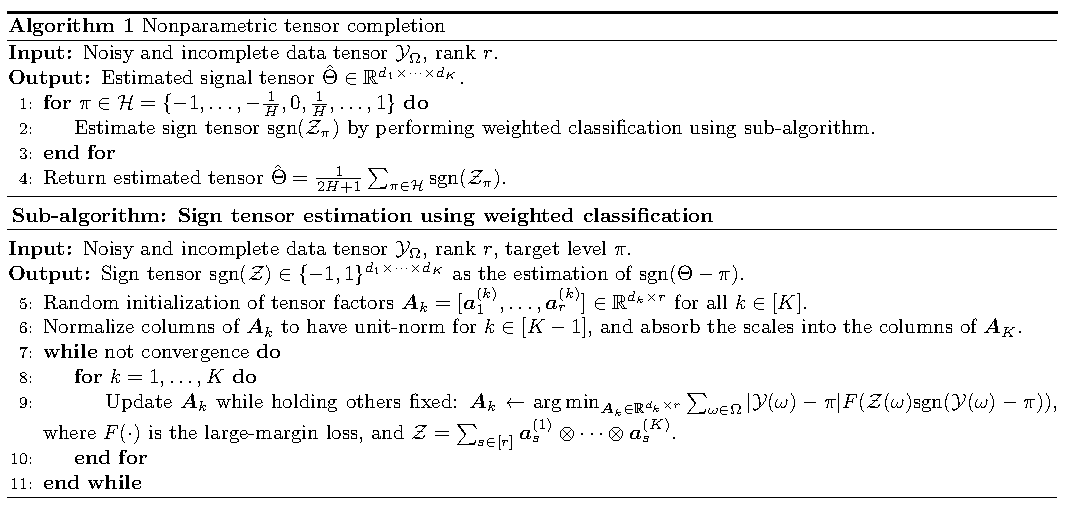
\includegraphics[width=\textwidth]{figure/algorithm.pdf}
\vspace{-.8cm}
\end{figure*}

 \begin{thm}[Sign tensor errors]\label{thm:classification} Suppose $\Theta\in\caliP(r)$ and $\Theta(\omega)$ is $\alpha$-globally smooth under $\omega\sim \Pi$, where $\alpha\in(0,1]$. Let $\hat \tZ_\pi$ be the estimator in~\eqref{eq:estimate}, and denote $d_{\max}=\max_{k\in[K]} d_k$. Then, for all $\pi\in[-1,1]$ except for a finite number of levels, with very high probability over $\tY_\Omega$, 
\begin{align}\label{eq:bound}
\textup{MAE}(\sign \hat \tZ_\pi, \sign(\Theta-\pi)) \lesssim & \left({d_{\max} r \over |\Omega|}\right)^{\alpha\over \alpha+2}\notag \\
&+{1 \over \rho^2(\pi, \tN)} {d_{\max}r \over |\Omega|}.
\end{align}
\end{thm}
Theorem~\ref{thm:classification} provides the error bound for the estimated sign tensors. Compared to the population version results in Theorem~\ref{thm:population}, we here explicitly reveal the dependence of accuracy on the sample complexity and on the level $\pi$. The result~\eqref{eq:bound} shows the sign error decreases with $|\Omega|$, provided that $\alpha \neq 0$. In particular, our sign estimate achieves consistent recovery using as few as $\tilde O(d_{\max}r)$ noisy observations. 
%In the case of equal dimension and full observation $|\Omega|=d^K$, the sign estimate reaches a fast rate $d^{-(K-1)}$ when $\alpha=\infty$. 


Combining the sign representability of the signal tensor and the sign estimation accuracy, we obtain the main results on our nonparametric tensor estimation method.
\begin{thm}[Tensor estimation error]\label{thm:estimation} Consider the same conditions of Theorem~\ref{thm:classification}. Let $\hat \Theta$ be the estimate in~\eqref{eq:est}. With very high probability over $\tY_\Omega$,
\begin{equation}\label{eq:bound}
\textup{MAE}(\hat \Theta, \Theta)\lesssim \left({d_{\max} r \over |\Omega|}\right)^{\alpha/(\alpha+2)}+{1\over H}+H{d_{\max} r \over |\Omega|}.
\end{equation}
In particular, setting $\scriptstyle H\asymp \left( |\Omega|\over d_{\max}r\right)^{1/2}$ yields the error bound
\begin{equation}\label{eq:real}
\textup{MAE}(\hat \Theta, \Theta)\lesssim \left(d_{\max}r \over|\Omega|\right)^{{\alpha \over \alpha+2} \vee {1\over 2}}.
\end{equation}
\end{thm}
Theorem~\ref{thm:estimation} demonstrates the convergence rate of our tensor estimation. The bound~\eqref{eq:bound} reveals three sources of errors: the estimation error inherited from sign tensors, the bias from sign series representations, and the variance thereof. The resolution parameter $H$ controls the bias-variance tradeoff. We remark that the signal estimation error~\eqref{eq:real} is generally no better than the corresponding sign error~\eqref{eq:bound}. This is to be expected, since magnitude estimation is a harder problem than sign estimation. 

In the special case of full observation with equal dimension $d_1=\cdots=d_K=d$, our signal estimate achieves convergence rate
\begin{equation}
\textup{MAE}(\hat \Theta, \Theta)\leq \left(r\over d^{K-1}\right)^{{\alpha \over \alpha+2} \vee {1\over 2}}.
\end{equation}
In contrast to earlier methods, our estimation accuracy applies to both low- and high-rank signal tensors $\Theta$. The rate depends on the sign complexity $\Theta\in\caliP(r)$, and this $r$ is often much smaller than the usual tensor rank (see Section~\ref{sec:sign-rank}). Therefore, our method not only incorporates the earlier work on low-rank tensor estimation but also addresses a broad family that was previously impossible. 

We apply our method to selected examples in Section~\ref{sec:sign-rank}, and compare the results with existing literature. The numerical comparison is provided in Section~\ref{sec:simulation}. 
\begin{customexample}{2}[Tensor block models]
Consider a tensor block model with $r$ multiway blocks in total. Our result implies a rate $\tO(d^{-(K-1)/2})$ by taking $\alpha=\infty$. This rate agrees with the  previous root-mean-square error (RMSE) for block tensor estimation~\cite{wang2019multiway}.
\end{customexample}

\begin{customexample}{3} [CP/Tucker and GLMs] 
Consider a GLM tensor $\Theta=g(\tZ)$, where $g$ is a known link function and $\tZ$ is a latent low-rank tensor. Suppose the marginal density of $\Theta(\omega)$ is bounded from above. Applying our results with $\alpha=1$ yields $\tO(d^{-(K-1)/3})$. Note that this rate is slightly slower than the parametric RMSE rate~\cite{zhang2018tensor,wang2018learning}. One possible reason is that our result remains valid for unknown $g$ and more general high-rank tensors with $\alpha=1$. The tensor family involved in our upper bound is broader than parametric models. 
\end{customexample}

The following sample complexity for nonparamtric tensor completion is a direct consequence of Theorem~\ref{thm:estimation}. 
\begin{cor}[Sample complexity for nonparametric completion] Under the same conditions of Theorem~\ref{thm:estimation}, with very high probability over $\tY_\Omega$, 
\[
\textup{MAE}(\hat \Theta, \Theta)\to 0, \quad \text{as}\quad {|\Omega|\over {d_{\max}} r}\to \infty.
\]
\end{cor}
Our result improves earlier work~\cite{ghadermarzy2019near} by allowing both low- and high-rank signals. Note that $\tilde \tO(d_{\max}r)$ roughly matches the degree of freedom in sign tensors, suggesting the optimality of our sample complexity. 


\begin{figure*}[h!]
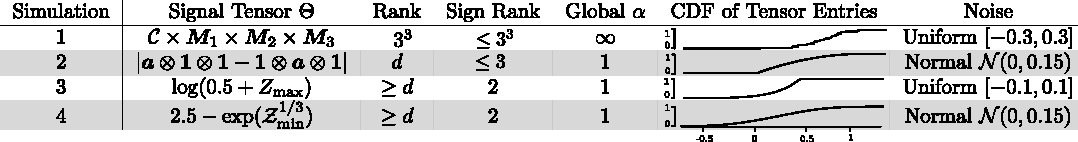
\includegraphics[width=1\textwidth]{figure/simulation_new.pdf}
\vspace{-.8cm}
\caption{Simulation models used for comparison. We use $\mM_k\in\{0,1\}^{d\times 3}$ to denote membership matrices, $\tC\in\mathbb{R}^{3\times 3\times 3}$ the block means, $\ma={1\over d}(1,2,\ldots,d)^T \in\mathbb{R}^d$, $\tZ_{\max}$ and $\tZ_{\min}$ are order-3 tensors with entries ${1\over d}\max(i,j,k)$ and ${1\over d}\min(i,j,k)$ respectively.}\label{tab:simulation}
\vspace{-.4cm}
\end{figure*}


\subsection{Numerical implementation}
This section addresses the practical implementation of our estimation~\eqref{eq:est} illustrated in Figure~\ref{fig:demo}. Our sign representation of tensor estimate $\Theta$ is a simple average of $H$ sign tensors, which can be solved in a divide-and-conquer fashion. Briefly, we estimate the sign tensors $\tZ_\pi$ (which are detailed in the next paragraph) for the series $\pi \in \tH$ through parallel implementation, and then aggregate the results for the final output. This approach maintains low computational cost similar to a single sign tensor estimation.  


For the sign tensor estimation~\eqref{eq:estimate}, the problem reduces to binary tensor decomposition with a weighted classification loss. A number of algorithms have been developed for this problem~\cite{ghadermarzy2018learning,wang2018learning,hong2020generalized}. We adopt similar ideas by tailoring the algorithms to our contexts. Following the common practice in classification, we replace the binary loss $\ell(z,y)=|\sign z - \sign y|$ with a surrogate loss $F(m)$ as a continuous function of margin $m\stackrel{\text{def}}{=}z\sign(y)$. Examples of large-margin loss are hinge loss $F(m) = (1-m)_+$, logistic loss $F(m) =\log(1+e^{-m})$, and nonconvex $\psi$-loss $F(m)=2\min(1,(1-m)_+)$ with $m_{+}=\max(m,0)$. We implement the hinge loss and logistic loss in our algorithm, although our framework is applicable to general large-margin losses~\citep{bartlett2006convexity}. 


The rank constraints in the optimization~\eqref{eq:est} have been extensively studied in literature. Recent developments involve convex norm relaxation~\cite{ghadermarzy2018learning} and nonconvex optimization~\cite{wang2018learning, han2020optimal}. Unlike matrices, computing the tensor convex norm is NP hard, so we choose (non-convex) alternating optimization due to its numerical efficiency. Briefly, we use the rank decomposition~\eqref{eq:CP} of $\tZ=\tZ(\mA_1,\ldots, \mA_K)$ 
%\mA_K)=\sum_{s=1}^r\ma^{(1)}_s\otimes \cdots \otimes \ma^{(K)}_s$ write the optimization~\eqref{eq:estimate} as
%\begin{align}
%\min_{\mA_k\colon k\in[K]}&\sum_{\omega\in \Omega}|\tY-\pi|F(\tZ(\omega)\sign(\tY(\omega)-\pi)),\\
%\text{subject to }\tZ&=\tZ(\mA_1,\ldots,\mA_K)=\sum_{s=1}^r\ma^{(1)}_s\otimes \cdots \otimes \ma^{(K)}_s,
%\end{align}
where $\mA_k=[\ma^{(k)}_1,\ldots,\ma^{(k)}_r]\in\mathbb{R}^{d_k\times r}$ are unknown factor matrices to optimize. We numerically solve \eqref{eq:est} by optimizing one factor $\mA_k$ at a time while holding others fixed. Each suboptimization reduces to a convex optimization with a low-dimensional decision variable. Following common practice in tensor optimization~\cite{anandkumar2014tensor,hong2020generalized}, we run the optimization from multiple initializations to locate a final estimate with the lowest objective value. The full procedure is described in Algorithm 1.

\section{Simulation}\label{sec:simulation}
In this section, we compare our nonparametric tensor method ({\bf NonParaT}) with two alternative approaches: low-rank tensor CP decomposition ({\bf CPT}), and the matrix analogy of our method applied to tensor unfolding ({\bf NonParaM}). We assess the performance under both complete and incomplete observations. The signal tensors are generated based on four models listed in Table~\ref{tab:simulation}. The simulation covers a wide range of complexity, including block tensors, transformed low rank tensors, min/max hypergraphon with log and exponential functions. We consider order-3  tensors of equal dimension $d_1=d_2=d_3=d$, and set $d\in \{15, 20,\ldots,55,60\}$, $r=2$, $H=10+{(d-15)/ 5}$ in Algorithm 1. For {\bf NonParaM}, we apply Algorithm 1 to each of the three unfolded matrices and report the average error. All summary statistics are averaged across $30$ replicates.  


\begin{figure}[h!]
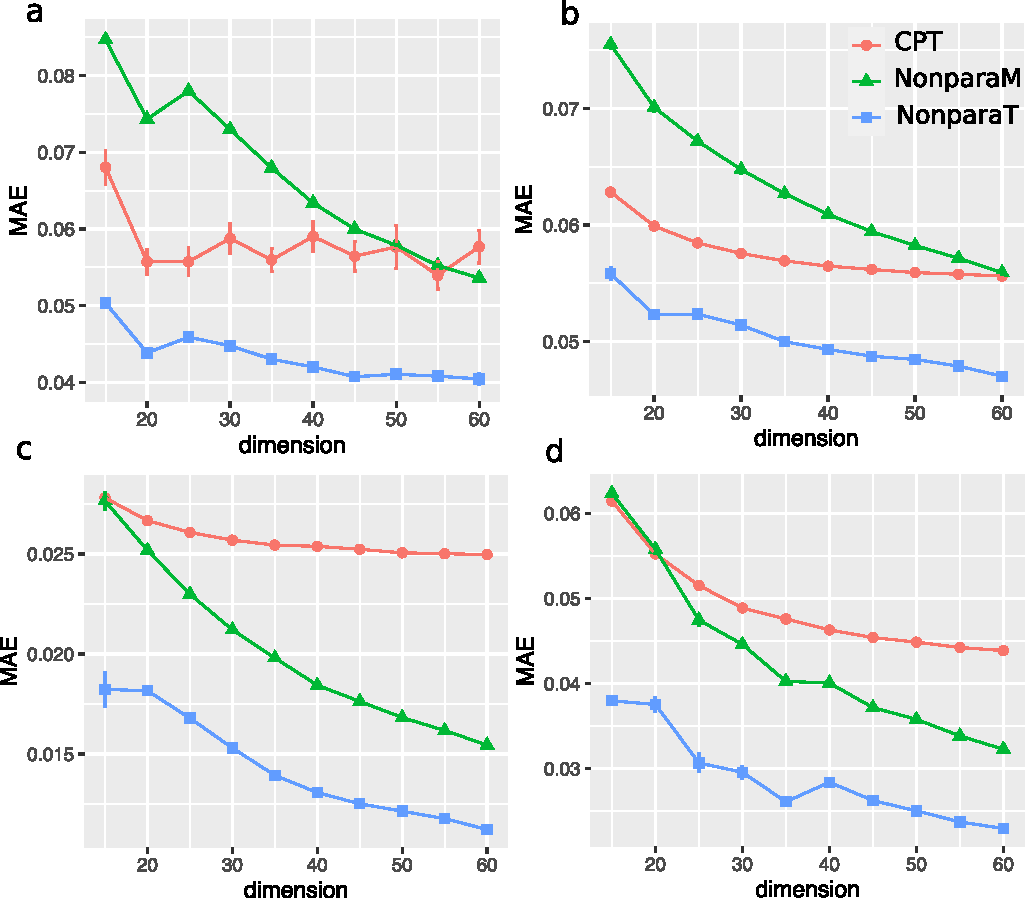
\includegraphics[width=.45\textwidth]{figure/fig1-4.pdf}
\vspace{-.4cm}
\caption{Estimation performance against tensor dimension. Panels (a)-(d) correspond to simulation models 1-4 in Table~\ref{tab:simulation}.}\label{fig:compare1}
\vspace{-.2cm}
\end{figure}


Figure~\ref{fig:compare1} compares the estimation error with full observation. We find all three methods show decreased error as the dimension increases. Furthermore, our method {\bf NonParaT} achieves the best performance in all scenarios, whereas the second best method is {\bf CPT} for models 1-2, and {\bf NonParaM} for models 3-4. One possible reason is that models 1-2 have controlled multilinear tensor rank, which makes tensor methods {\bf NonParaT} and {\bf CPT} more accurate than matrix methods. For models 3-4, the rank exceeds the tensor dimension, and the two nonparametric methods {\bf NonParaT} and {\bf NonparaM} are well suited for high rank signals. 

%The result also demonstrates the robustness of our method to various shapes of $\Theta(\omega)$. As we shown in Section~\ref{sec:identifiability}, the CDF of $\Theta(\omega)$ plays a key role in estimation accuracy, and a jump at $\pi$ makes $\pi$-weighted classification hard. Nevertheless, we find that our method maintains good performance in model 1 where the signal tensor $\Theta(\omega)$ has $3^3$ many jumps. The reason of this robustness is that we aggregate in total $(2H+1)$ sign tensors, each of which incurs at most ${1\over H}$ error to the final tensor estimate. Therefore, the estimation is robust against a few off-target sign tensor estimations, as long as the majority are accurate.  


Figure~\ref{fig:compare2} shows the completion error against observation fraction. We fix $d=40$ and gradually increase the observation fraction ${|\Omega|\over d^3}$ from 0.3 to 1. It is seen that {\bf NonParaT} achieves the lowest error among all methods. Our simulation covers a reasonable range of various complexities; %for example, the CDF of $\Theta()$model 1 has $3^3$ jumps, the 
%and the improved accuracy highlights the ability of our nonparametric method in tensor completion. 
%We point out that the simulated models do not necessarily satisfy our method assumptions. 
for example, model 1 has $3^3$ jumps in the CDF of signal $\Theta$, and models 2 and 4 have unbounded noise. Nevertheless, our method shows good performance in spite of model misspecification. This result is appealing in practice because the structure of underlying signal tensor is often unknown. 

\begin{figure}[h!]
\vspace{-.2cm}
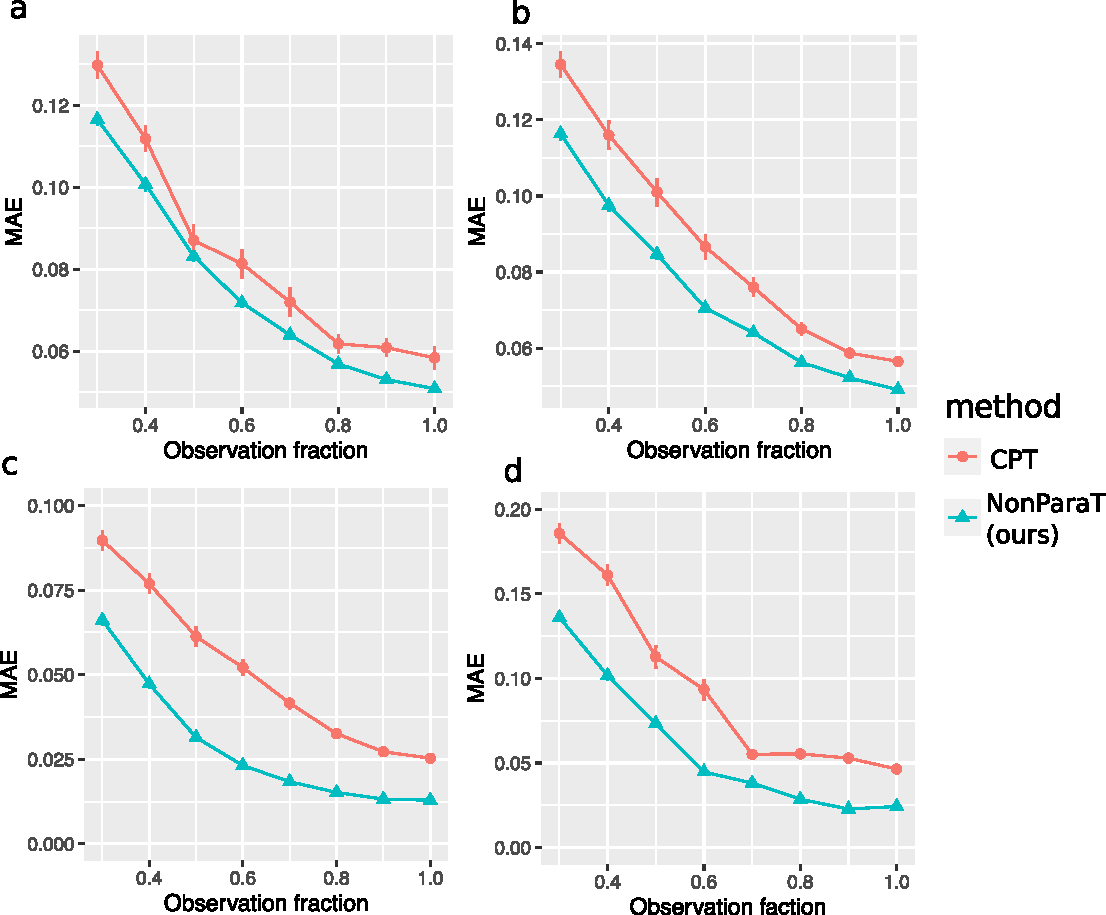
\includegraphics[width=.45\textwidth]{figure/fig5-8.pdf}
\vspace{-.2cm}
\caption{Completion performance against observation fraction. Panels (a)-(d) correspond to simulation models 1-4 in Table~\ref{tab:simulation}. }\label{fig:compare2}
\vspace{-.4cm}
\end{figure}

\section{Data analysis}
We apply our method to two tensor datasets, the MRN-114 human brain connectivity data~\citep{wang2017bayesian}, and NIPS data~\cite{globerson2007euclidean}. The MRN-144 dataset records the structural connectivity among 68 brain regions for 114 individuals along with their Intelligence Quotient (IQ) scores. We organize the connectivity data into an order-3 tensor, where entries encode the presence or absence of fiber connections between brain regions across individuals. The NIPS dataset consists of counts of words in NIPS papers published from 1987 to 2003. We focus on the top 100 authors, 200 most frequent words, and normalize each word count by log transformation with pseudocount 1. The resulting dataset is an order-3 tensor with entry representing the log counts of words by authors across years. 

\begin{table}[h!]
\vspace{-.1cm}
\resizebox{.45\textwidth}{!}{
\begin{tabular}{c|c|c|c}
\Xhline{2\arrayrulewidth}
\multicolumn{4}{c}{MRN-144 brain connectivity dataset}\\
\Xhline{2\arrayrulewidth}
Method                    & $r=6$ &  $r=9$&$r=12$\\
\hline
NonparaT (Ours)  & {\bf 0.14}(0.003) &  {\bf 0.12}(0.004)&{\bf 0.12}(0.007)\\
CPT  & 0.23(0.006)&0.22(0.004)&0.21(0.004)\\
 \Xhline{2\arrayrulewidth}
\multicolumn{4}{c}{NIPS dataset}\\
 \Xhline{2\arrayrulewidth}
Method                    & $r=6$& $r=9$&$r=12$\\
\hline
NonparaT (Ours)  & {\bf 0.16}(0.002)& {\bf 0.15}(0.001)&{\bf 0.14}(0.001)\\
CPT &0.20(0.007)&0.19(0.007)&0.17(0.007)
%Naive imputation &\multicolumn{2}{c}{0.32(.001)}
\end{tabular}
}
\vspace{-.2cm}
\caption{Comparison of prediction error in the MRN-114 and NIPS data analysis. For low-rank CPT, we use R function {\tt rTensor} with default hyperparameters, and for our method, we set $H = 20$.}\label{tab:data}
\vspace{-.2cm}
\end{table}


Table~\ref{tab:data} compares the prediction accuracy of our method and low-rank CP method. The reported MAE is averaged over five runs of cross-validation, with 20\% entries for testing and 80\% for training. Our method substantially outperforms the classical low-rank method for every configuration in the considered range. Further increment of rank appears to have little effect on the performance, and we find that increased missingness gives more advantages to our method (see details in Appendix). In contrast, the low-rank CPT exhibits poor prediction even at a relatively high rank. The comparison highlights the advantage of our method in achieving accuracy while maintaining low complexity. 

\begin{figure}[h!]
\vspace{-.3cm}
\centering
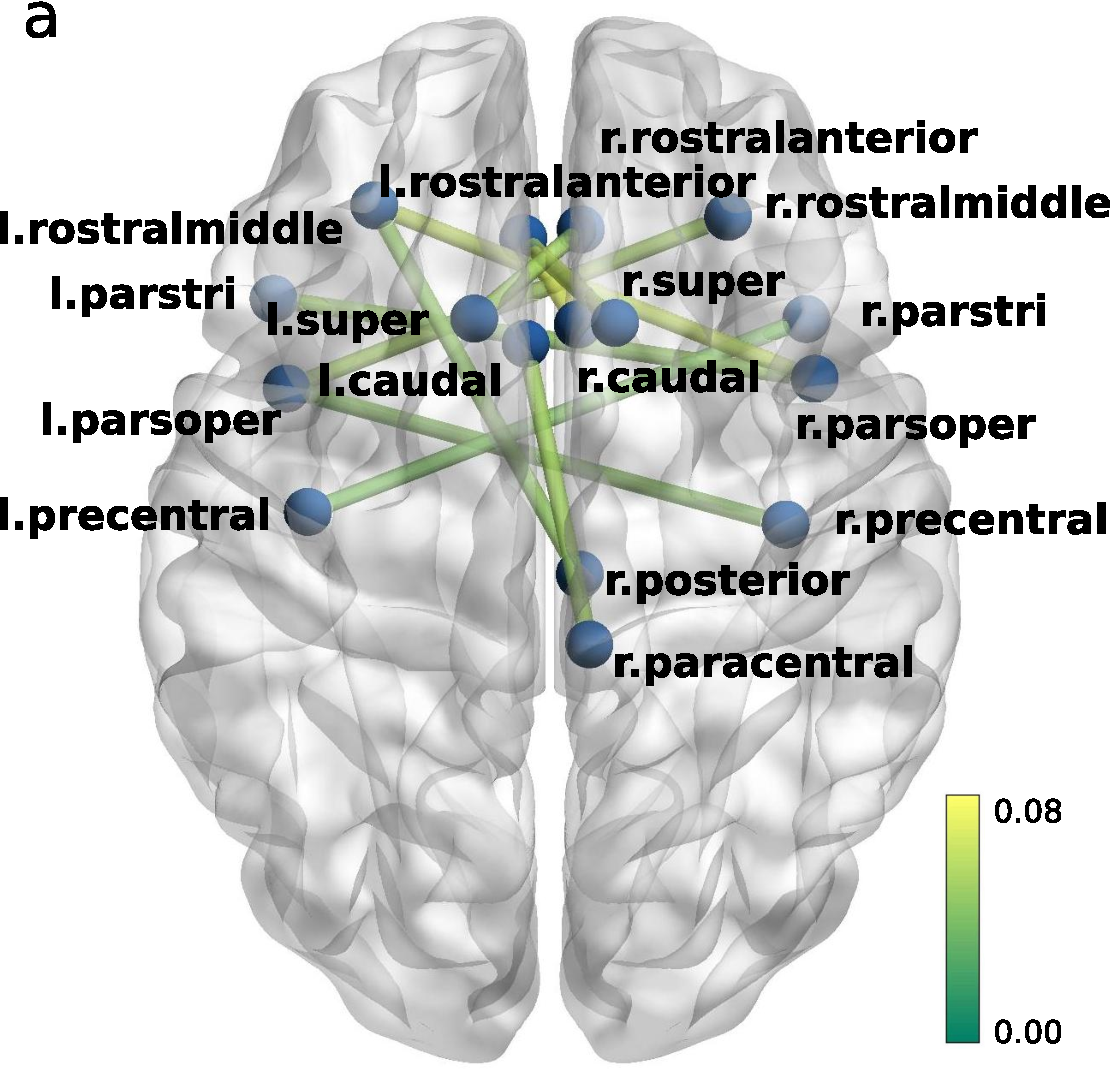
\includegraphics[width=.2\textwidth]{figure/brainIQ.pdf}
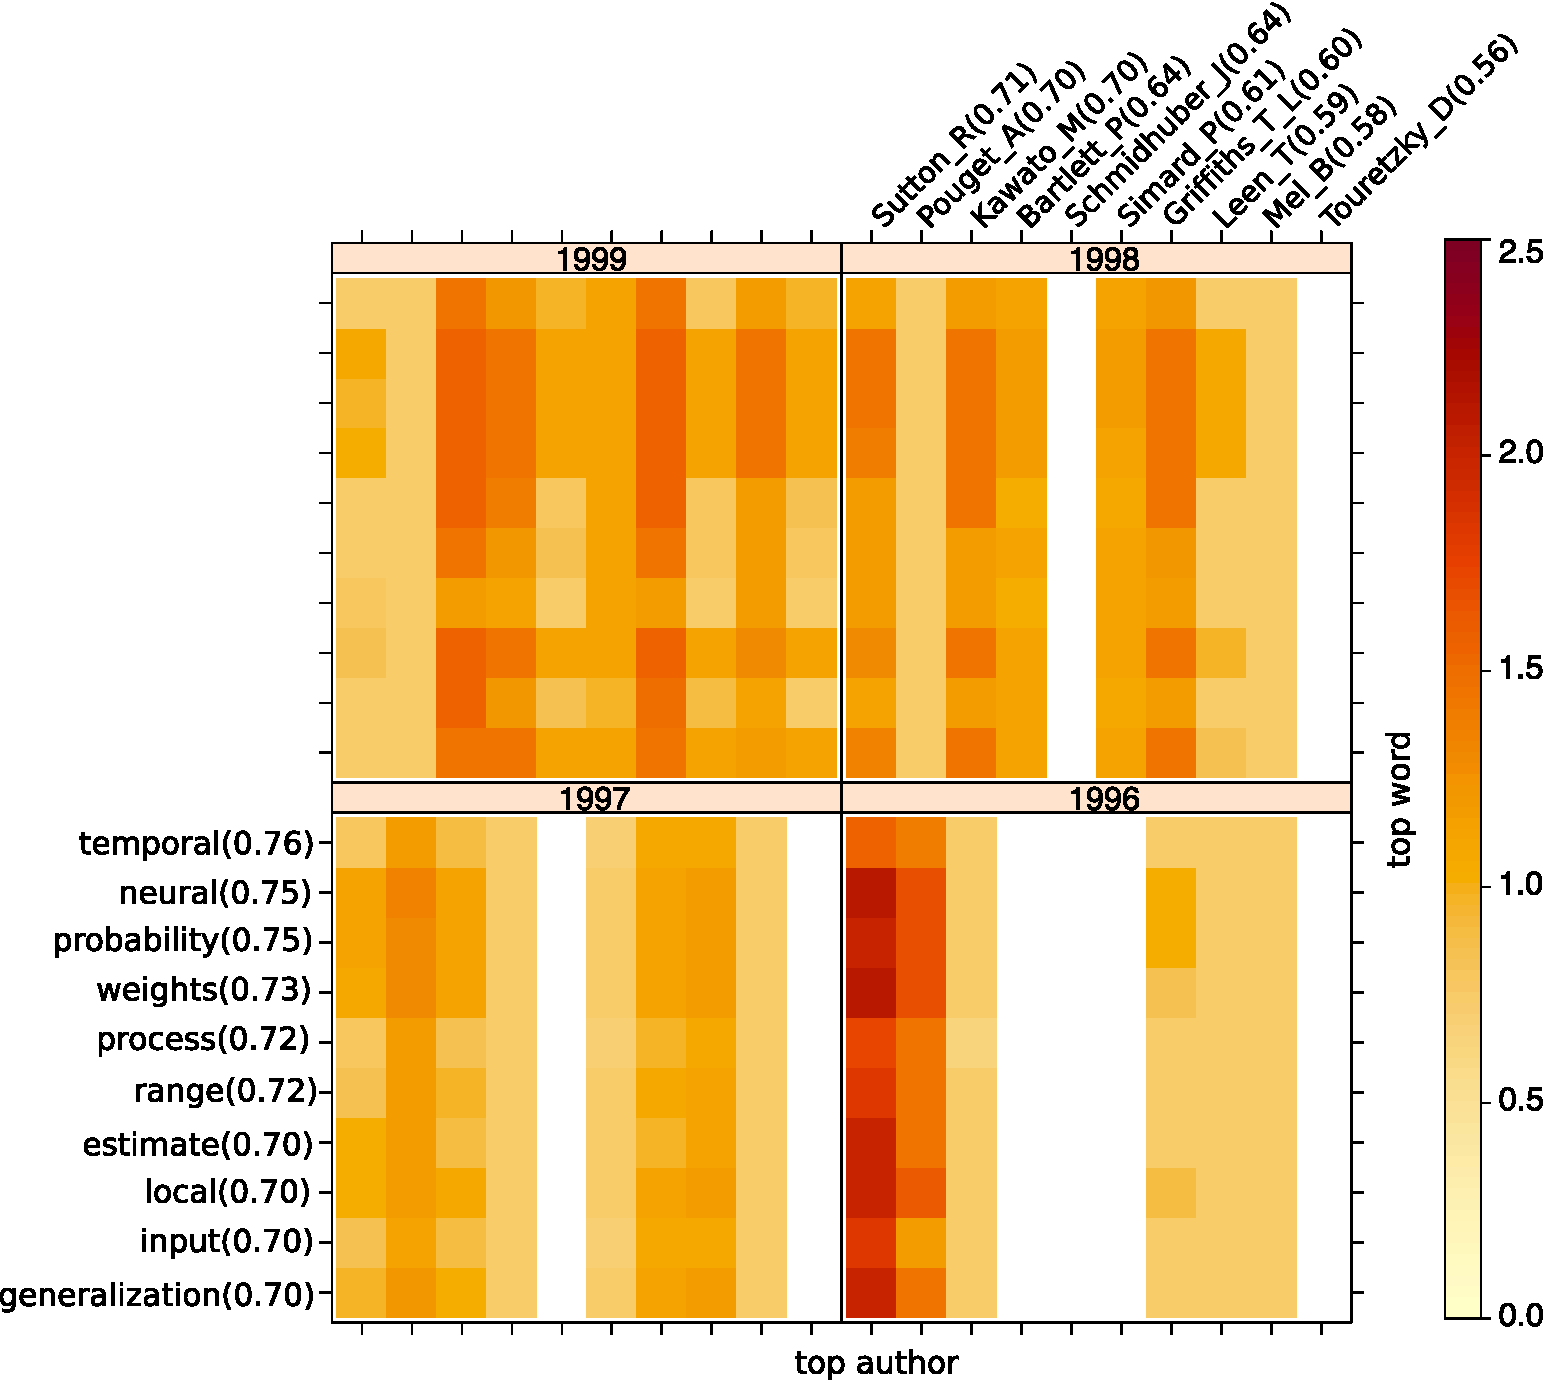
\includegraphics[width=.27\textwidth]{figure/signal.pdf}
\caption{Estimated signal tensor from brain connectivity data (a) and NIPS data (b). %Authors and words are ranked by marginal averages based on $\hat \Theta$, where the marginal average is denoted in the parentheses.
}\label{fig:signal}
\vspace{-.3cm}
\end{figure}

We next examine the estimated signal tensor $\hat \Theta$ form our method. Figure~\ref{fig:signal}a shows the top 10 edges in MSN-144 dataset based on regression analysis of denoised edge connection with IQ scores. We find that top edges are mostly inter-hemisphere, which are consistent with recent research in brain connectivity pattern with intelligence~\cite{li2009brain,wang2017bayesian}. Figure~\ref{fig:signal}b illustrates the result from NIPS data, where we plot the top entries in $\hat \Theta$ corresponding to top authors and words (after excluding generic words such as \emph{figure}, \emph{current}, etc). The detected patten is consistent with the active topics in the NIPS publication. Among the top words are \emph{temporal} (marginal mean = 0.76), \emph{neural} (0.75), and \emph{generalization} (0.70), whereas top authors are \emph{Richard Sutton} (0.71), \emph{Pouget\_A}(0.70), \emph{Kawato\_M} (0.70), and \emph{Bartlett Peter} (0.64). We also find strong heterogeneity among word occurrence across authors and years. For example, \emph{neural} and \emph{weights} are popular words for \emph{Tomas Griffiths} in 1998-1999, whereas \emph{temproal} occurs more often in \emph{Richard Sutton et al} in 1996. The achieved denoising accuracy and pattern detection demonstrates the applicability of our method.


\section{Conclusion}
We have developed high-rank tensor estimation based on sign series representation. Our work offers a new paradigm for structure learning, and we obtain results that were previously hard to establish. Tensor learning is a great challenge for further research. We hope the work opens up new inquiry that allow more researchers to contribute to this field.


\bibliographystyle{chicago}

\bibliography{tensor_wang}

\appendix

\end{document}
